\chapter{Oscilloscope: User level concepts}
    The following chapter gives insights on the user level concepts of $\Delta$QSD in the oscilloscope. They are the concepts needed by the user to understand how the oscilloscope works.
    \begin{itemize}
        \item We first provide insights into how the concepts related $\Delta$QSD are implemented in the oscilloscope, the parameters that define a probe's $\Delta$Q, its representation. We show how probe's $\Delta$Q(s) will be shown in the oscilloscope.
        \item We then provide a language to write outcome diagrams based on an already existing syntax and provide an example.
        \item Lastly, we explain the different widgets on the oscilloscope dashboard and the available triggers.
    \end{itemize}

\section{$\Delta$QSD concepts}

    We provide in this section the concepts needed to understand what is displayed on the oscilloscope.

\subsection{Representation of a $\Delta$Q}
    We provide a class to calculate the $\Delta$Q of a probe between a lower time bound $t_l$ and an upper time bound $t_u$. It can be calculated in two ways: 
    
    \paragraph{Observed $\Delta$Q}
    
    The first way is by having $n$ collected outcome instances between $t_l$ and $t_u$, calculating its \textit{probability density function} (PDF) and then calculating the \textit{empirical cumulative distribution function} (ECDF) based on its PDF. This is called the \textbf{Observed $\Delta$Q}.
    
    \paragraph{Calculated $\Delta$Q}
    
    A $\Delta$Q can also be calculated by performing operations on two or more observed $\Delta$Qs (convolution, operators operations), the notion of outcome instances is then lost between calculations, as the interest shifts towards calculating the resulting PDFs and ECDFs. This is called the \textbf{Calculated $\Delta$Q}. A simple outcome can \textbf{not} have a "calculated $\Delta$Q", we can only observe the delay from its observables.

    If you recall \cref{fig:probes_o}, the probes $p_2$ and $p_3$ observe simple outcomes, they can only display the observed $\Delta$Qs of $o_2, o_3$. The probe $p_1$ instead observes the sequential composition of said outcomes. We can display its "observed $\Delta$Q" from the execution from $start$ to $end$ and the "calculated $\Delta$Q" as the convolution of the observed $\Delta$Qs of $o_1, o_2$
        
    \begin{figure}[H]
            \begin{center}
                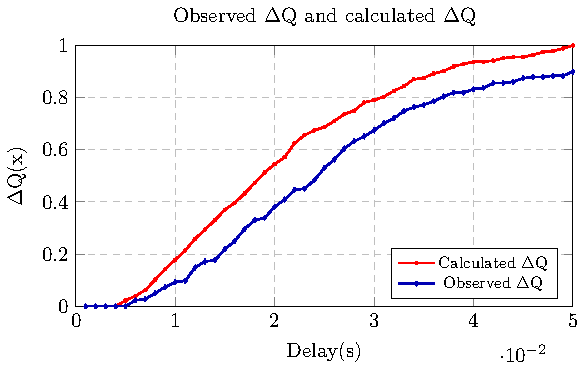
\includegraphics[scale=1]{tikz/obs_calc.pdf} 
            \end{center}
            \caption{(Red, circle, above): Calculated $\Delta$Q. (Blue, diamond, below): Observed $\Delta$Q}
        \end{figure}

    \subsection{dMax = $\Delta$t $\cdot$ N}
        The key concept of $\Delta$QSD is having a maximum delay after which we consider that the execution is timed out. This is represented in the oscilloscope as $dMax$. Understanding this equation is key to correctly using the oscilloscope and exploring tradeoffs

Setting a maximum delay for a probe is not a job that can be done one-off and blindly, it is something that is done with an underlying knowledge of the system inner-workings and must be thoroughly fine-tuned during the execution of the system by observing the resulting distributions of the obtained $\Delta$Qs. 

Let us explain the following equation:
\begin{equation}
    dMax = \Delta t \cdot N  
    \label{eq:dMaxU}
\end{equation}

    \begin{itemize}
        \item $dMax$: The maximum delay, it represents the maximum delay that an outcome instance of a probe can have. The execution is considered "timed out" (failure) after $dMax$.
        \item $\Delta t$: The resolution of a $\Delta$Q. It is the bin width of a bin in a probe's $\Delta$Q.
        \item $N$: The precision of a $\Delta$Q. It is the number of bins in a probe's $\Delta$Q.
    \end{itemize}
    
    It can be informally described as a "two out of three" equation. If the user wants higher precision but the same $dMax$, the resolution must change, and so on for every parameter.
        \begin{figure}[H]
            \centering
            \begin{subfigure}{.5\textwidth}
                \centering
                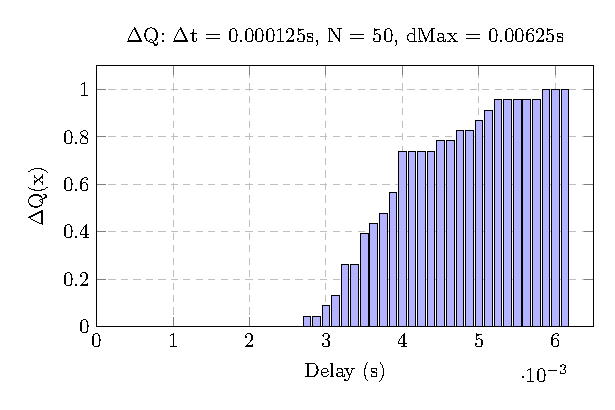
\includegraphics[width =0.98\textwidth]{tikz/hist_50.pdf}
                \label{fig:hist_50}
            \end{subfigure}%
            \begin{subfigure}{.5\textwidth}%
                \centering%
                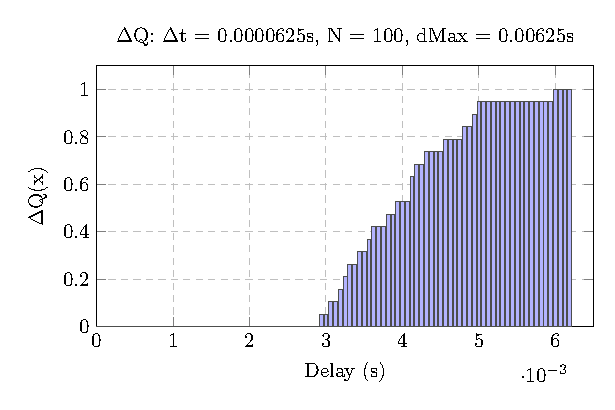
\includegraphics[width =0.98\textwidth]{tikz/hist_100.pdf}%
                \label{fig:hist_100}%
            \end{subfigure}%
            \label{fig:hist_dmax}%
            \caption{Left: Sample $\Delta$Q representation as a histogram with higher resolution but lower precision. \\
            Right: Sample $\Delta$Q representation as a histogram with lower resolution but higher precision. \\
            Both $\Delta$Qs have the same $dMax$, but the amount of precise information they provide is far different.}
        \end{figure}%

Some tradeoffs must though be acknowledged when setting these parameters, a higher number of bins corresponds to a higher number of calculations and space complexity, a lower $dMax$ may correspond to more failures. The user must set these parameters carefully during execution y observing the shown plots.

    \begin{figure}[H]
        \begin{center}
            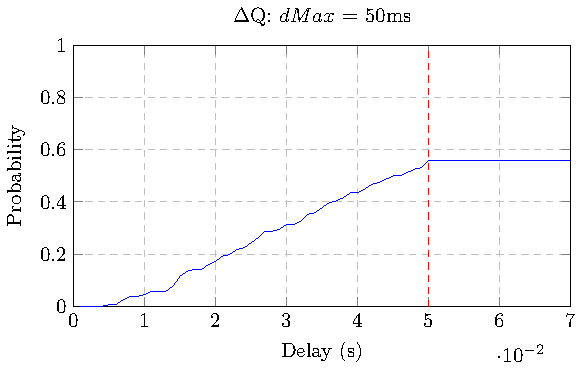
\includegraphics[scale = 1]{tikz/cdf_dmax.pdf}
        \end{center}
        \caption{$\Delta$Q: $dMax$ = 50ms, the $\Delta$Q will stay constant when delay $> dMax$.}
    \end{figure}

    \subsubsection{dMax limitation}
        $dMax$ can \textbf{not} be lower than 1 millisecond and will be rounded to the \textbf{nearest} integer in the adapter, this is a limitation of Erlang \texttt{send\_after} function which only accepts integers and milliseconds values. For example, if on the oscilloscope the $dMax$ is equal to $1.56 ms$, the adpater will fail spans after 2 ms.

    \subsection{QTA}
        A simplified QTA is defined for probes. We define 4 points for the step function at 25, 50, 75 percentiles and the maximum amount of failures accepted for an observable. An observed $\Delta$Q will calculate that based on the samples collected. 

\subsection{Confidence bounds}
    To observe the stationarity of a probe we must observe its $\Delta$Qs over a polling window and calculate confidence bounds over said $\Delta$Qs. A single $\Delta$Q may fluctuate, moreover, as it is an ECDF, it is not as precise as a CDF and, based on the number of bins, may not be precise. This is why we include the mean and confidence bounds of $\Delta$Qs in the plot.

    We first calculate a mean of the $\Delta$Qs in the polling window, this gives an idea of how the probe has been behaving during the polling window. \\
    Given this mean, we can calculate its confidence bounds, which give a probability range over which the true CDF of the $\Delta$Q should fall. \cite{conf-b}

    The bounds are updated dynamically by inserting or removing a $\Delta$Q. Every time a new $\Delta$Q is calculated, the oldest $\Delta$Q in a window is removed if \#$\Delta$Qs(polling window) $>$ limit. The new $\Delta$Q is added to the calculation of the mean and confidence bounds as it is calculated. \\
    This allows us to consider a small window of execution rather than observing the execution since the start for the bounds, this can help in observing stationarity of the system, where less sampled $\Delta$Qs can help observe short term behaviour. \\
    With a big window of $\Delta$Qs, temporary overload may not greatly affect the mean and bounds, while, if we consider the current size of the polling window (30 $\Delta$Qs), a few $\Delta$Qs which deviate from stationary behaviour have a greater impact on the bounds and mean.
        \begin{figure}[H]
            \begin{center}
                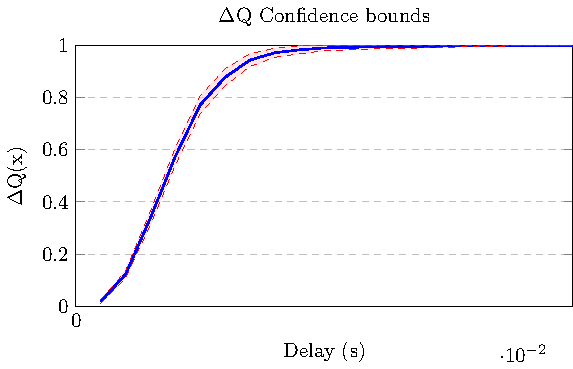
\includegraphics[scale=1]{tikz/ci.pdf} 
            \end{center}
            \caption{Upper and lower bounds (dashed, red) of the mean (blue) of multiple $\Delta$Qs. In a system that behaves linearly, the bounds will be close to the mean, once the overload is approaching, or a system is showing behaviour that diverges from a linear one, the bounds will appear larger.}
        \end{figure}

  

\section{$\Delta$Q display}
    Now that we have introduced the required concepts, we can put everything together to be plotted. In summary, a probe's displayed graph must contain the following functions:
    \begin{itemize}
        \item The observed $\Delta$Q of the sampling window, with the mean and confidence bounds of the polling window $\Delta$Qs.
        \item If applicable, the calculated $\Delta$Q from the causally linked components observed in a probe, with the mean and confidence bounds of the polling window $\Delta$Qs.
        \item Its QTA (if defined).
    \end{itemize}
    This allows for the user to observe if a $\Delta$Q has deviated from normal execution, analyse its stationarity, nonlinearity and observe its execution.

    In the photo below we can observe the multiple elements as they are displayed in real time in the oscilloscope.
    \begin{itemize}
        \item (1): The mean of the polling window observed $\Delta$Qs (yellow) with the confidence bounds of the mean. Upper bound (dark green) and lower bound (light green). The observed $\Delta$Q of the sampling window can be observed going out of the confidence bounds at delay 0.00125 s. The $\Delta$Q in a sampling window as is less precise than the mean and confidence bounds calculated in the polling window.
        \item Arrow, red, above: The mean of the calculated $\Delta$Qs (ochre) with the confidence bounds of the mean. Upper bound (purple) and lower bound (magenta). The calculated $\Delta$Q of the sampling window is inside its confidence bounds.
        \item (3): The \textbf{QTA}.
    \end{itemize}
     \begin{figure}[H]
        \begin{center}
            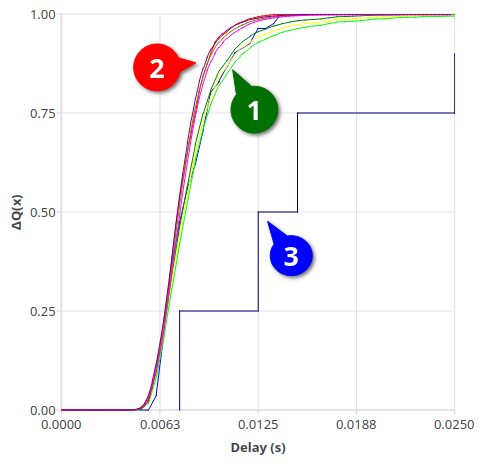
\includegraphics[scale = 0.7]{img/overload_2/fired_sampleb.png}
        \end{center}
         \caption{$\Delta$Qs, confidence bounds, means and QTA for a probe observing the causal link of multiple components.}
    \end{figure}
        


\section{Outcome diagram} \label{out_syntax}
        An abstract syntax for constructing outcome diagrams has already been defined in a previous paper \cite{art}, nevertheless, the oscilloscope needs a textual way to define an outcome diagram. \\ 
        We define  a grammar to create an outcome diagram in our oscilloscope, which is a textual interpretation of the abstract syntax.
        
      
        \subsection{Causal link}
            A causal link between two components can be defined by a right arrow from \texttt{component\_i} to \texttt{component\_j}:
        \begin{minted}{text}
            component_i -> component_j 
        \end{minted}
        
        \subsection{Sub-outcome diagrams}
            Multiple sub-outcome diagrams can be created for multiple parts of the system. They can then be linked together to form the global system outcome diagram. Sub-outcome diagrams can observe one or multiple components.
        Recall \cref{fig:probes_o}, we defined a probe which observes the sequential composition of $o_1, o_2$. The probe (sub-outcome diagram) $p_1$ can be defined as:
        \begin{minted}{text}
            p_1 = o_1 -> o_2;
        \end{minted}

        A probe is attached at the start and end events of $p_1$, it will observe the whole system and the calculated $\Delta$Q will be the convolution of $o_1, o_2$.

        The lines defining these diagrams must be semicolon terminated. Outcomes and operators cannot be defined on their own, they must be observed in a sub-outcome diagram.
        
        Sub-outcome diagrams can be reused in other diagrams by adding \texttt{s:} (sub-outcome diagram) before they are used.

            \begin{minted}{text}
                p_3 = s:p_1 -> s:p_2;
            \end{minted}
            This allows for easy composition and reuse of different parts of the system, allowing for independent refining of diagrams.

        \subsection{Outcomes}
            To attach a probe to an outcome observables, it is enough to declare an outcome with its name inside a diagram.
                \begin{minted}{text}
                    ... = outcomeName;
                \end{minted}
        \subsection{Operators}
            First-to-finish, all-to-finish and probabilistic choice operators must contain at least two components.
              \subsubsection{All-to-finish operator}
            An all-to-finish operator needs to be defined as follows:
            \begin{minted}{text}
                a:name(component1, component2...)
            \end{minted}

        \subsubsection{First-to-finish operator}
            A first-to-finish operator needs to be defined as follows:
            \begin{minted}{text}
                f:name(component1, component2...)
            \end{minted} 

        \subsubsection{Probabilistic choice operator}
            A probabilistic choice operator needs to be defined as follows:
            \begin{minted}{text}
                p:name[probability_1, probability_2, ... probability_i](component_1, component_2, ..., component_i) 
            \end{minted}
            In addition to being comma separated, the number of probabilities inside the brackets must match the number of components inside the parentheses. For $n$ probabilites $p_i$, $0 < p_i < 1$, $\sum_{i = 0}^{n} p_i = 1$ 
        
            
        \subsection{Limitations}
            Our system has a few limitations compared to the theoretical applications of $\Delta$Q, namely, no cycles are allowed in the definition of outcome diagrams. 
        
        \begin{minted}{text}
            p_1 = s:p_2;
            p_2 = s:p_1;
        \end{minted}
        The above example is not allowed and will raise an error when defined.  

    \subsection{Outcome diagram example}
        We provide a sample example of an outcome diagram definition. We also provide its resulting outcome diagram with probes inserted.
        \begin{figure}[H]
        \begin{minted}{text}
            two_hops = o2 -> o3;
            total = p:pc[0.9, 0.1](o1, s:two_hops);
        \end{minted}
            \caption{Sample textual definition of an outcome diagram.}
        \label{fig:outcd}
        \end{figure}

        \begin{figure}[H]
            \begin{center}
                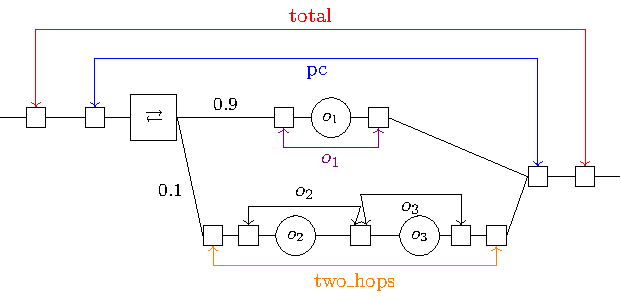
\includegraphics[scale=1.3]{tikz/system.pdf}
            \end{center}
            \caption{Resulting outcome diagram for definition \ref{fig:outcd}.}%
        \end{figure}

\section{Dashboard}
    The dashboard is devised of multiple sections where the user can interact with the oscilloscope, create the system, observe the behaviour of its components, set triggers.

    \subsection{Sidebar}
        The sidebar has multiple tabs, we explain here the responsibility of each one.

    \subsubsection{System/Handle plots tab}

    \paragraph{System creation}
        In this tab the user can create its system using the grammar defined before, he can save the text he used to define the system or load it, the system is saved to a file with any extension, we nevertheless define an extension to save the system to, the extension \texttt{.dq}.
        If the definition of the input is wrong, he will be warned with a pop-up giving the error the parser generator encountered in the creation of a system.

    \paragraph{Adding a plot}
        Once the system is defined, the user can choose the probes he wants to plot. They can select multiple probes per plot and display multiple plots on the oscilloscope window.
    
    \paragraph{Sampling rate}
        The user can choose the sampling rate of the system: How often $\Delta$Qs are calculated and displayed in the oscilloscope.

    \paragraph{Editing a plot}
        By clicking onto a plot that is being shown, the user can choose to add or remove probes to and from it, thanks to the widget in the lower right corner. Multiple probes can be selected to either be removed or added.

    \subsubsection{Parameters tab}
        In this tab, the user can define parameters for the probes they have defined.

    \paragraph{Set a QTA}
        The user is given the choice to set a QTA for a given probe, they have 4 fields where they can fill in which correspond to the percentiles and the maximum amount of failures allowed, they can change this dynamically during execution.

    \paragraph{dMax, bins}
        The user can set the parameters we explained previously, $\Delta$t and $N$. When this information is saved by the user, the new $dMax$ is transmitted to the adapter and saved for the selected observable.

    \subsubsection{Triggers tab}
        In the triggers tab the user can set triggers and observe the snapshots of the system.

    \paragraph{Set triggers}
        The user can set which triggers to fire for the probes they desire, they are given checkboxes to decide which ones to set as active or not (by default, the triggers are deactivated).
    
    \paragraph{Fired triggers}
        Once a trigger is fired, the oscilloscope starts a timer, during which all probes start recording the observed $\Delta$Qs (and the calculated ones if applicable) without discarding older ones. Once the timer expires, the snapshot is saved for the user in the triggers tab. In the dashboard, it indicates when the trigger was fired (timestamp) and the name of the probe which fired it.
   
   \subsubsection{Connection controls}
    
        \paragraph{Erlang controls}
            The user can set the IP and the port where the $\Delta$Q adapter is listening from. Two additional buttons communicate with the adapter by sending messages, they can start and stop the adapter's sending of outcome instances.
        
        \paragraph{C++ server controls}
            The user can set the IP and the port for the oscilloscope's server.

\subsection{Plots window}
        To the left, the main window shows the plots of the probes being updated in real time. 

\section{Triggers}
    There are two available triggers which can be selected by the user, the triggers are evaluated on the \textbf{observed $\Delta$Q}.

    Part of future work is extending the available triggers in the oscilloscope. We are aware that the number of available triggers may not seem like much. Nut the triggers we provide a sufficient basis to observe the non-linearity of a system and are sufficient to detect overload.
    \subsection{Load}
        A trigger on an observed $\Delta$Q \textit{of a sampling window} can be fired if the amount of outcome instances received for a probe in a sampling window is greater than what the user defines:
    \begin{center}
        \#instances$_{probe}$($\Delta$Q) > maxAllowedInstances$_{probe}$ 
    \end{center}

    \subsection{QTA}
        A trigger on an observed $\Delta$Q \textit{of a sampling window} can be fired if:
        \begin{center}
            $\Delta$Q$_{obs}$ $\nless$ observableQTA
        \end{center}


